% =====================================================================
%  The phase figure as it stood in each draft, panels (a) and (b), as a
%  standalone picture. The panels themselves come from fig_phaseclock.py,
%  which runs each draft's own generator in a throwaway worktree.
%  Build: make pairclock.pdf
% =====================================================================
\documentclass[border=8pt]{standalone}
\usepackage[T1]{fontenc}
\usepackage{lmodern}
\usepackage{graphicx}
\graphicspath{{fig/}}

\begin{document}
\begin{minipage}{17.6cm}
  \begin{minipage}[t]{0.515\linewidth}
    \centering
    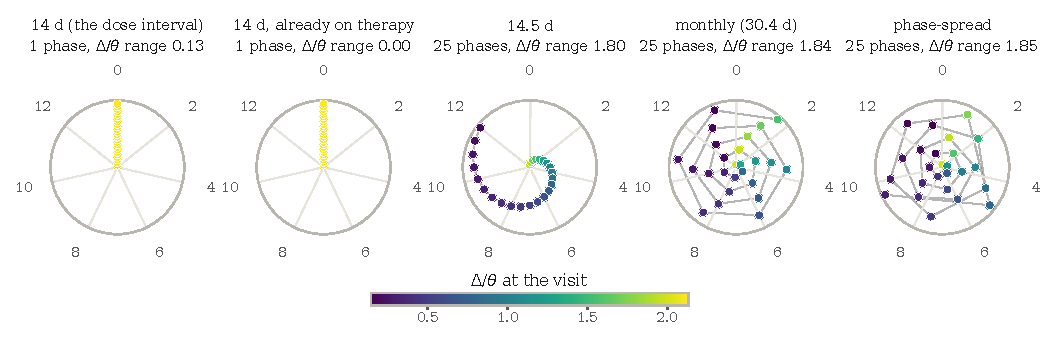
\includegraphics[width=\linewidth]{phaseclock_0920}\\[4pt]
    {\footnotesize (a) 20 Sept: polar dial, one spoke at the dose interval\par}
  \end{minipage}\hfill
  \begin{minipage}[t]{0.465\linewidth}
    \centering
    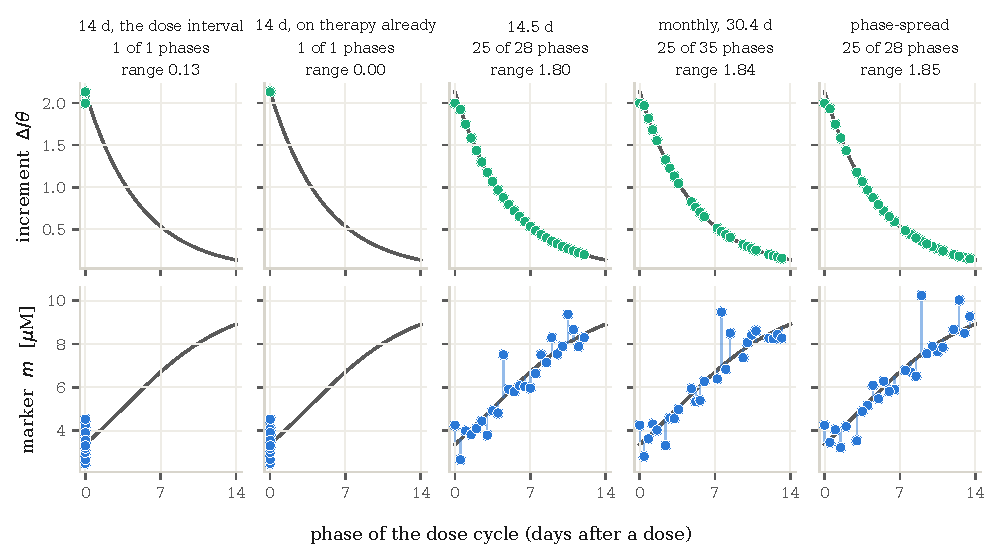
\includegraphics[width=\linewidth]{phaseclock_0927}\\[4pt]
    {\footnotesize (b) 27 Sept: increment and marker folded onto the cycle\par}
  \end{minipage}
\end{minipage}
\end{document}
